\documentclass[smallextended]{svjour3}
\usepackage{fix-cm}
\usepackage[T1]{fontenc}
\usepackage[utf8]{inputenc}
\usepackage{mathptmx}
\usepackage{amsmath,amssymb,graphicx,booktabs,tabularx,url}
\usepackage{placeins}
\usepackage[numbers,sort&compress]{natbib}
\usepackage[hidelinks]{hyperref}
\journalname{Computing}
\smartqed
\setlength{\emergencystretch}{2em}
\newcommand{\CollegePRDelta}{-0.90780}
\newcommand{\CollegePRLoss}{9.01}
\newcommand{\CollegePRSaving}{86.44}
\newcommand{\CollegePRfiveDelta}{-0.43094}
\newcommand{\CollegePRfiveLoss}{4.28}
\newcommand{\CollegePRfiveSaving}{82.83}
\newcommand{\CollegeDegreeDelta}{0.00000}
\newcommand{\CollegeDegreeLoss}{0.00}
\newcommand{\CollegeDegreeSaving}{86.59}
\newcommand{\GrqcPRDelta}{-0.25082}
\newcommand{\GrqcPRLoss}{5.07}
\newcommand{\GrqcPRSaving}{92.70}
\newcommand{\GrqcPRfiveDelta}{0.00000}
\newcommand{\GrqcPRfiveLoss}{0.00}
\newcommand{\GrqcPRfiveSaving}{88.14}
\newcommand{\GrqcDegreeDelta}{0.00000}
\newcommand{\GrqcDegreeLoss}{0.00}
\newcommand{\GrqcDegreeSaving}{92.77}
\newcommand{\WikiPRDelta}{-40.69334}
\newcommand{\WikiPRLoss}{73.01}
\newcommand{\WikiPRSaving}{96.42}
\newcommand{\WikiPRfiveDelta}{-13.53012}
\newcommand{\WikiPRfiveLoss}{24.28}
\newcommand{\WikiPRfiveSaving}{91.98}
\newcommand{\WikiDegreeDelta}{0.00000}
\newcommand{\WikiDegreeLoss}{0.00}
\newcommand{\WikiDegreeSaving}{96.26}

\begin{document}
\title{Evaluating Candidate-Restricted Influence Maximization: Reference Budgets, Ranking Precision, and External Topologies}
\titlerunning{Evaluating candidate-restricted influence maximization}
\author{\mbox{Jiayue Sun} \and \mbox{Binbin Yong} \and \mbox{Junjie An} \and \mbox{Tianyu Bo} \and \mbox{Shuai Li}}
\authorrunning{Jiayue Sun et al.}
\institute{Jiayue Sun \at School of Artificial Intelligence, Lanzhou University, Lanzhou 730000, China
\and Binbin Yong (corresponding author) \at School of Information Science and Engineering, Lanzhou University, Lanzhou 730000, China \\
\email{yongbb14@lzu.edu.cn}
\and Junjie An, Tianyu Bo and Shuai Li \at Lanzhou University, Lanzhou, China}
\date{}
\maketitle
\begin{abstract}
Restricting seed candidates reduces the cost of influence maximization, but its measured quality depends on both the sampled reference and the numerical ranking used to construct the pool. We develop a paired evaluation framework that separates these two resolutions and relates seed agreement to independent spread and computational cost. Experiments on three real network topologies use nested selection budgets, shared random worlds and independent spread evaluation; a post-hoc control isolates ranking precision. On ca-GrQc, default PageRank changes from a 5.61\% gain to a 5.07\% loss as the reference budget increases. Tightening the solver tolerance removes this reversal, while budget-dependent seed changes remain. At the highest tested budget, degree-based pools of 20 candidates reproduce all 15 full-greedy trajectories and reduce measured selection time by 98.40--99.67\% relative to exhaustive full-candidate selection. PageRank losses on the directed networks persist under tighter precision. These findings distinguish reference reproduction from utility preservation and identify budget, ranking precision and candidate coverage as necessary context for interpreting restriction quality.
\keywords{influence maximization \and Monte Carlo simulation \and candidate restriction \and evaluation methodology \and reproducibility}
\end{abstract}

\section{Introduction}
Candidate restriction reduces the search cost of greedy influence maximization by allowing only a subset of vertices to become seeds. The quality of that restriction is commonly judged against a full-candidate greedy reference. With a finite simulation budget, however, the reference is itself a sampled computation: increasing its budget can change the selected seeds and the apparent loss of a restricted method. Reproducing the reference, preserving independently evaluated spread and saving computation are therefore distinct outcomes.

A second source of variation arises before greedy selection. A numerical ranking can change only slightly while exchanging vertices at the candidate-pool boundary. Those exchanges can change the final seeds. Coverage and topology further complicate the comparison: a pool containing most of a small contact graph may contain less than one percent of a larger network, and incoming PageRank importance need not align with outgoing simulated spread.

Sampling accuracy and scalability are established concerns in influence maximization \cite{ref1,ref2,ref8,ref9,ref16}. We examine how reference budget and ranking precision jointly affect the evaluation of a truncated candidate pool. Our paired design holds the propagation graph, selection worlds and tie rule fixed across full and restricted greedy selection, then evaluates both seed sets on shared, independent worlds (Fig.~\ref{fig:evaluation-mechanism}). This design connects the source of a selection change to its utility and cost consequences.

The study provides three contributions:
\begin{itemize}
\item We identify a ranking-precision dependence in an apparent budget-induced quality reversal: tightening PageRank tolerance removes the ca-GrQc reversal, although budget-dependent seed changes persist.
\item We test the transfer of candidate-ranking results to three larger real topologies. Degree-based pools retain full-reference agreement at the highest tested budget, whereas PageRank's earlier contact-graph agreement does not transfer uniformly.
\item We quantify how reference-set changes translate into independent spread differences and how candidate restriction trades utility against measured selection cost.
\end{itemize}

\begin{figure}[t]
\centering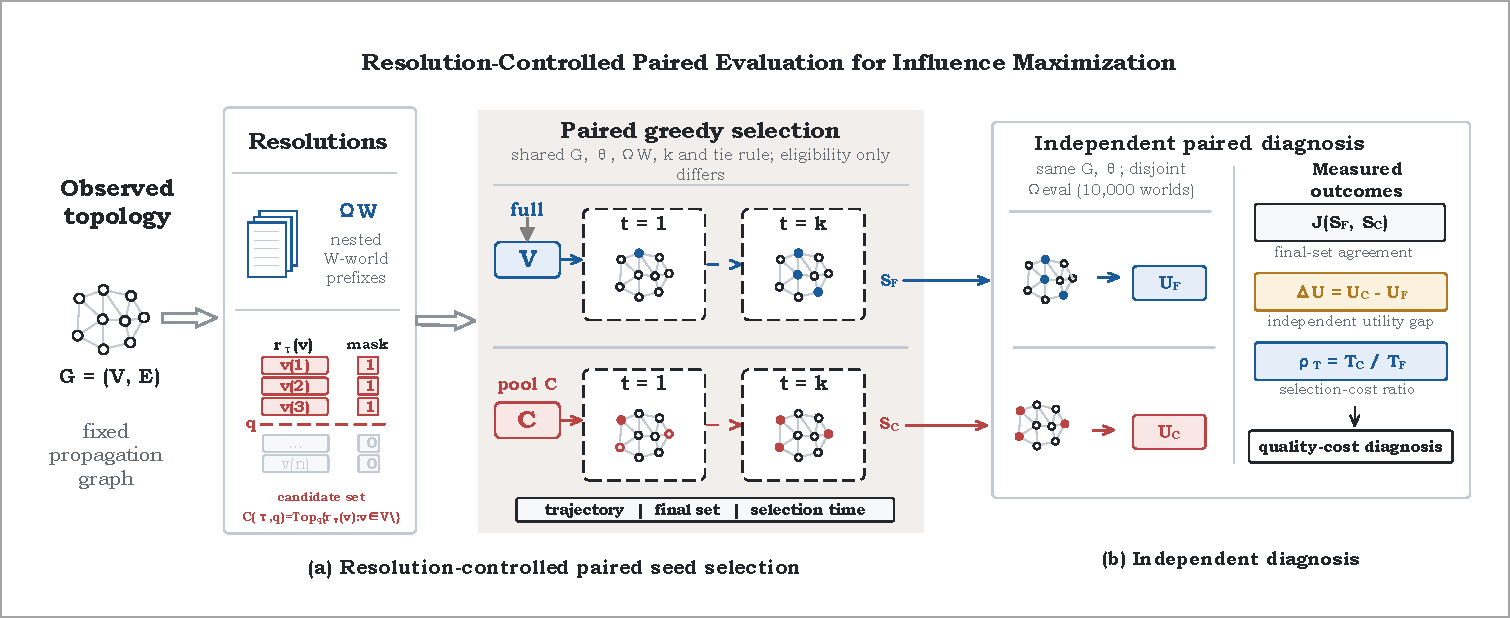
\includegraphics[width=\linewidth]{FigEvaluationMechanism.pdf}
\caption{Paired evaluation separates reference resolution, ranking resolution and restriction quality. (a) The selection budget $W$ and ranking tolerance $\tau$ determine the finite-world reference and the top-$q$ pool $C(\tau,q)$. Both arms share the graph, world prefix, seed budget and tie rule. (b) Shared evaluation worlds, independent of selection, yield the utility difference $\Delta U$. Set agreement $J$ and selection-cost ratio $\rho_T$ complete the quality--cost comparison.}\label{fig:evaluation-mechanism}
\end{figure}

\section{Related work}
Classical independent-cascade influence maximization connects expected spread to greedy seed selection \cite{ref1}. CELF reduces repeated marginal evaluations using objective structure \cite{ref7}; StaticGreedy reuses fixed realizations \cite{ref8}; IMM develops a sampling-based solver with approximation guarantees \cite{ref2}. These approaches motivate careful treatment of the sampled objective. We use exhaustive per-round enumeration to isolate the effect of seed eligibility under a common finite-world objective.

Ranking and search strategies offer complementary routes to efficient selection. Neighbour-scale centrality \cite{ref12} and discrete metaheuristic optimization \cite{ref13}, both studied in \emph{Computing}, change how influential seeds are identified. Learned inductive estimators such as MONSTOR+ predict spread on unseen graphs \cite{ref19}. Our comparisons retain one simulator and greedy rule while changing the candidate pool, allowing differences to be attributed to eligibility and evaluation resolution.

Benchmarking has established the importance of comparable models and implementation scope \cite{ref16}. Temporal-network formulations \cite{ref11} and empirical influence models \cite{ref15} also distinguish observed relations from diffusion assumptions. Our evidence concerns simulated spread on observed topologies. The evaluation jointly tracks reference budget, ranking precision, coverage, seed agreement, independent spread and cost. Online Resource 1 provides a source-scoped comparison of these dimensions.

\section{Methods}
\subsection{Paired selection at controlled resolutions}
Let $G=(V,E)$ be a directed propagation graph and $S$ a seed set of size $k$. Under the independent-cascade model, each newly activated vertex gets one opportunity to activate each inactive outgoing neighbour with probability $p$. Propagation stops after $h$ rounds. For a random world $\omega$, let $f_h(S;\omega)$ denote total activated vertices, including seeds. Greedy selection uses the sampled objective
\begin{equation}
\widehat\sigma_W(S)=\frac{1}{W}\sum_{w=1}^{W}f_h(S;\omega_w).
\end{equation}
At each round, greedy selection enumerates every unselected eligible vertex and chooses the largest integer total $W\widehat\sigma_W$. Ties resolve by lexicographic original node ID. Full selection uses $C=V$; restricted selection uses $C\subseteq V$. All vertices remain in the propagation graph. Both arms share $G$, the world prefix, $k$ and the tie rule.

We vary reference resolution through $W$ and ranking resolution through the numerical tolerance $\tau$. Degree ranks distinct outgoing neighbours. PageRank uses the unweighted directed topology and NetworkX 3.5 defaults: damping .85, uniform personalization and dangling-node treatment, tolerance $10^{-6}$ and at most 100 iterations \cite{networkxpr}. Its stopping criterion is successive-vector $L_1$ change below $n\tau$, where $n=|V|$. Scores are sorted decreasingly with lexical ties. A top-$q$ pool contains $q=\min(n,4k)$ or $q=\lceil .05n\rceil$ vertices. Historical weighted degree counts outgoing observed events where such counts exist. Three random pools are independently generated within each graph/path and fixed across budgets and coupling controls.

\subsection{World coupling and independent evaluation}\label{sec:coupling}
Primary selection worlds share draws indexed by world, propagation step, source and target. This coupling preserves the independent-cascade marginal law for each fixed seed set, but the realized finite-world objective can be nonmonotone. For example, initially activating an intermediate vertex can move its outgoing attempt to an earlier step with a different sampled outcome. Online Resource 1 gives the explicit counterexample. A separate fixed-edge control draws once per edge and world; its finite objective is coverage by vertices reachable within $h$ edges and is monotone and submodular. Both implementations use exhaustive enumeration.

Selection-world identifiers form nested prefixes as $W$ increases. Evaluation uses a disjoint family of $M=10,000$ worlds per path, shared by all seed sets and held fixed across budgets. Keys also separate graphs, paths and candidate-pool randomization. Coupling schemes are compared within their own full references.

For restricted seeds $S_C$ and full-reference seeds $S_F$, define the paired evaluation difference on world $i$ as $d_i=f_h(S_C;\eta_i)-f_h(S_F;\eta_i)$. The utility gap in Fig.~\ref{fig:evaluation-mechanism} is
\begin{equation}
\widehat\Delta=\frac{1}{M}\sum_{i=1}^{M}d_i,
\qquad \operatorname{SE}_{\rm MC}=s(d_i)/\sqrt M.
\end{equation}
The interval $\widehat\Delta\pm1.96\operatorname{SE}_{\rm MC}$ describes conditional Monte Carlo uncertainty for fixed selected sets. Across-path standard deviation describes variation across computational paths, including finite evaluation noise. The three random-pool evaluation vectors are averaged within each path before either calculation.

We report ordered-trajectory agreement, final-set agreement, Jaccard similarity and the first divergent round. Incremental spread subtracts $k$ from total spread; percentage incremental loss is $-100\widehat\Delta/(\widehat\sigma_{\rm full}-k)$. Negative loss favors the restricted set. All observed denominators are positive. The frozen primary tests compare degree-4k, PageRank-4k and the within-path random mean with full selection at $W=1280$, using two-sided exact sign tests and Holm correction across three comparisons within each graph. Zero differences are excluded and reported. Coverage, coupling and transition analyses are descriptive; worlds and paths are not independent network samples.

\subsection{Implementation and cost measurement}
The Numba implementation stores candidate IDs, selected sequences, integer round totals and per-world evaluation values. Audits verify source/data/result hashes, reconstruct argmax and tie decisions, replay full scores and evaluations, and compare predetermined worlds with a separate scalar oracle. Identical seed sets must yield identical evaluation vectors. The source snapshots, audit qualifications and reproducible commands accompany Online Resource 1.\footnote{OpenAI Codex assisted code, verification, analysis, figure generation and drafting. The authors reviewed the outputs and take responsibility for the manuscript.}

Selection time includes greedy search and lexical candidate sorting, but excludes graph preparation, world generation and evaluation. We additionally report a warm-process verification-inclusive estimate: separately measured parsing, graph construction and one method's ranking/pool generation are added to the frozen selection-world, selection, evaluation-world and evaluation times. Setup uses the median of five repeats. These assembled estimates exclude imports, just-in-time compilation, downloads and output writing. Five randomized repeats at path 1101 and $W=320$ assess timing variability. Cost comparisons use this implementation's exhaustive full-candidate reference; strict-tolerance results are used only for quality sensitivity, not the default-tolerance timing comparison.

\section{Experimental setup}
\subsection{Networks and preprocessing}
We selected three larger SNAP topologies before inspecting seed sets or utilities \cite{snap}: CollegeMsg communication, ca-GrQc collaboration and wiki-Vote voting. Table~\ref{tab:data} reports the processed sizes and candidate coverage. All retained components are included.
\begin{table}[htbp]
\caption{Processed external networks and candidate coverage. Arcs are directed propagation arcs; the 5\% pool contains $\lceil .05n\rceil$ vertices.}\label{tab:data}
\begin{tabular}{lrrrr}
\toprule
Graph & Nodes & Arcs & 4k fraction & 5\% pool \\
\midrule
CollegeMsg & 1,438 & 13,397 & 1.391\% & 72 \\
ca-GrQc & 5,241 & 28,968 & 0.382\% & 263 \\
wiki-Vote & 7,115 & 103,689 & 0.281\% & 356 \\
\bottomrule
\end{tabular}
\end{table}

CollegeMsg records timestamped sender-to-receiver messages \cite{college}. We retain the first 65\% of complete timestamp groups, yielding 38,939 non-self events. Historical weighting counts outgoing messages, while propagation uses uniform $p$ on distinct directed pairs. ca-GrQc links coauthors \cite{grqc}; we remove self-loops, deduplicate pairs and create reciprocal arcs. Vertices are collected after loop removal, excluding the self-loop-only vertex 12295 and giving 5,241 rather than the source page's 5,242 vertices. wiki-Vote arcs run from voter to votee \cite{signed,links}. Outgoing diffusion on these arcs is a simulation assumption. The two static datasets supply neither event counts nor observed cascades and receive no historical-weighted ranking. Exact timestamps, graph hashes and component counts are in the supplementary records.

Historical context comes from four contact-derived graphs with 75--402 vertices, constructed from workplace, conference and rural Kenya data \cite{ref3,ref4,ref5,ref6}. The initial 42-condition study is distinct from a later 520-condition extension with ten paths per real graph, selection budgets up to 5120 and two 2,000-node synthetic controls based on preferential attachment and stochastic blocks \cite{ref17,ref18}. Their complete configurations and results remain separate from the external study.

\subsection{Primary matrix and numerical sensitivity control}
The main external setting fixes $k=5$, $p=.01$ and $h=3$. Three graphs, five paths (1101--1105) and $W=80,320,1280$ define 45 step-coupled conditions. Nine fixed-edge conditions use $W=320$ and paths 1101--1103. Every condition includes full selection, degree-4k, PageRank-4k, degree-5\%, PageRank-5\% and three random-4k pools; CollegeMsg also includes historical-weighted 4k and 5\% pools. All 54 conditions and 468 arms were completed and retained. Resource preflight recorded timing and memory only and is excluded from utility evidence.

A post-hoc numerical control tightens PageRank tolerance to $10^{-12}$ with at most 1,000 iterations. Its two protocols were frozen before the corresponding new utility outputs: the first covers $W=1280$, and the second adds $W=80,320$. Together they contain 45 conditions and 90 restricted arms, reusing the original five paths, full references and evaluation worlds. All strict pools agree with those at $10^{-14}$. This paired sensitivity analysis adds no independent paths and leaves the primary test family unchanged.

\section{Results}
\subsection{External topology changes the ranking comparison}
At $W=1280$, degree-4k reproduces every full-greedy trajectory across the three external graphs using only 20 candidates (Table~\ref{tab:primary}). Default PageRank-4k matches none and incurs mean incremental losses of \GrqcPRLoss{}\%, \CollegePRLoss{}\% and \WikiPRLoss{}\% on ca-GrQc, CollegeMsg and wiki-Vote. The historical extension showed much broader PageRank agreement: 40/40 trajectories at $W=5120$, compared with 39/40 for degree. The external results therefore limit transfer of the contact-graph ranking result.
\begin{table}[htbp]
\caption{External results at $W=1280$ (five paths). PageRank (PR) and degree use 20-node pools; PR uses default tolerance. Loss is relative to full incremental spread. Degree agreement counts identical ordered trajectories.}\label{tab:primary}
\begin{tabular}{lrrrr}
\toprule
Graph & Full spread$^a$ & PR gap & PR loss (\%) & Degree$^b$ \\
\midrule
ca-GrQc & 4.934 & -0.25082 & 5.07 & 5/5 \\
CollegeMsg & 10.072 & -0.90780 & 9.01 & 5/5 \\
wiki-Vote & 55.736 & -40.69334 & 73.01 & 5/5 \\
\bottomrule
\end{tabular}
\par\smallskip\footnotesize $^a$Incremental spread (nodes). PR gap is also in nodes. $^b$Trajectory matches out of five paths.
\end{table}


Every primary PageRank and random-mean path difference is negative, giving unadjusted sign-test $p=.0625$ and within-graph Holm $p=.1875$. Degree differences are exactly zero. Five paths limit the minimum two-sided sign-test value to .0625; these results establish neither statistical equivalence nor absence of loss. Effect magnitudes and sensitivity controls provide the main basis for interpretation. Online Resource 1 retains the complete matrix, random-pool results and tests.

\subsection{Ranking precision resolves an apparent budget reversal}
Figure~\ref{fig:precision-budget} separates the effects of selection budget and ranking precision. On ca-GrQc, default PageRank-4k changes from a 5.61\% gain at $W=80$ to losses of 2.53\% and 5.07\% at 320 and 1280. Tightening tolerance exchanges two of 20 candidates and yields gains of 11.25\%, 2.96\% and 0.54\%. The original gain-to-loss reversal thus depends on the numerical ranking.

Budget still matters under the stable strict pool. Its selected sets change on 3/5 paths from 80 to 320 and 2/5 from 320 to 1280. At $W=1280$, the mean paired difference is only $+0.02608$ nodes, with path values from $-0.0408$ to $+0.1789$ and path standard deviation 0.09155. The mean gain is small relative to this variation. A change in sign alone would obscure that scale.

CollegeMsg's default and strict pools, seeds and evaluations are identical at every budget, retaining losses of 9.33\%, 8.52\% and 9.01\%. On wiki-Vote, one candidate changes, but strict losses remain 74.05\%, 74.05\% and 73.96\%. Precision sensitivity is therefore network-specific: it changes the ca-GrQc interpretation while preserving the two directed-network losses.
\begin{figure}[t]
\centering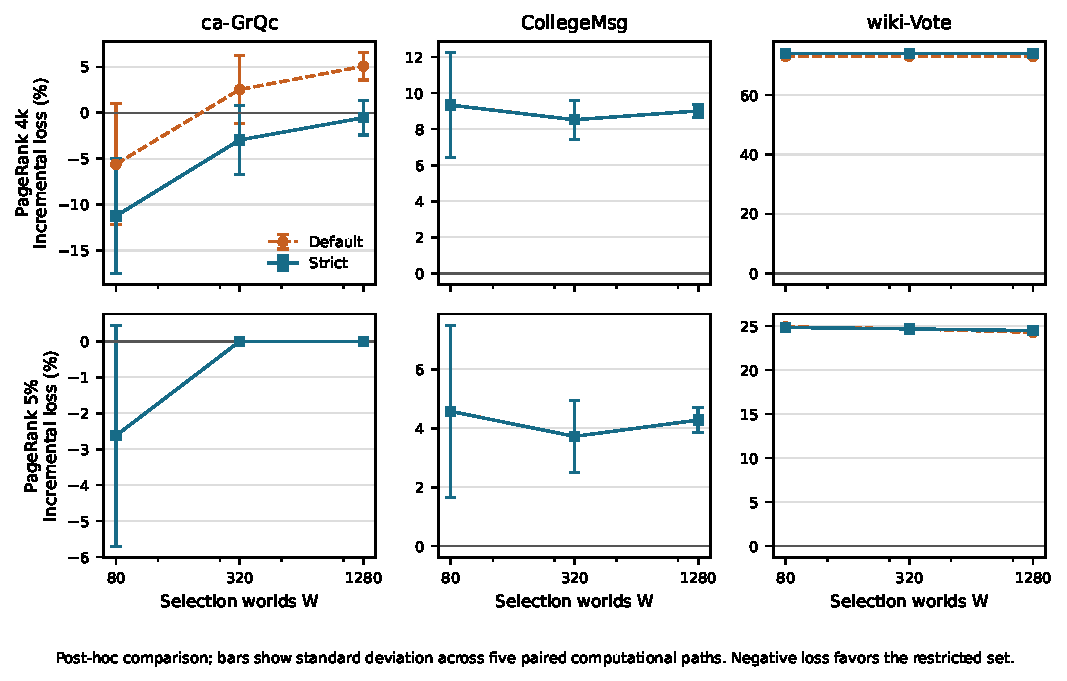
\includegraphics[width=\linewidth]{Fig4.pdf}
\caption{Budget and ranking precision have distinct effects on candidate-restriction quality. Points are mean incremental losses over five paired paths; bars are path standard deviations. Default and strict tolerances are $10^{-6}$ and $10^{-12}$, with strict pools stable at $10^{-14}$. Negative loss favors the restricted set. The ca-GrQc default reversal disappears under strict ranking, while the directed-network losses persist. This is a post-hoc paired sensitivity analysis.}\label{fig:precision-budget}
\end{figure}

\subsection{Coverage and direction qualify the loss interpretation}
Increasing the default PageRank pool to 5\% reproduces all five ca-GrQc references at $W=1280$ and reduces CollegeMsg loss from \CollegePRLoss{}\% to \CollegePRfiveLoss{}\%. On wiki-Vote, loss falls from \WikiPRLoss{}\% to \WikiPRfiveLoss{}\%, but remains substantial. Historical-weighted CollegeMsg pools similarly improve from a mean difference of $-0.25224$ nodes at 4k to exact reference reproduction at 5\%. Coverage helps in these comparisons, but its effect differs across networks.

The wiki-Vote structural diagnostic connects poor coverage to ranking orientation. The default PageRank top 20 have mean in-degree 249.75 and out-degree 56.2; the degree top 20 have mean in-degree 70.3 and out-degree 489.25. The PageRank-4k pool contains none of the five full-reference seeds on any $W=1280$ path, and its 5\% pool contains only one. These observations are consistent with a mismatch between incoming importance and outgoing propagation. Direction was not experimentally reversed, so the diagnostic does not isolate a causal mechanism. The seed-level illustration and complete coverage comparisons appear in Online Resource 1.

\subsection{Changed reference sets can have small utility differences}
Figure~\ref{fig:transitions} compares reference-set changes with independent utility changes. From $W=320$ to 1280, all five ca-GrQc sets change, but their mean gain is 0.12720 nodes; individual differences range from $-0.0266$ to $+0.2411$. CollegeMsg changes one set and gains 0.05336 nodes averaged across all five paths. wiki-Vote changes no final sets and has exactly zero paired gain, although some ordered sequences change.

Of the six changed sets, four have positive pointwise 95\% conditional Monte Carlo intervals; two ca-GrQc intervals include zero. The nine unchanged sets have identical evaluation vectors. These comparisons separate the occurrence of a selection change from its size and direction in utility. The historical 1280-to-5120 comparison reinforces this distinction: 16/40 sets changed while mean gain was 0.01111 nodes, without establishing convergence on the external networks.
\begin{figure}[t]
\centering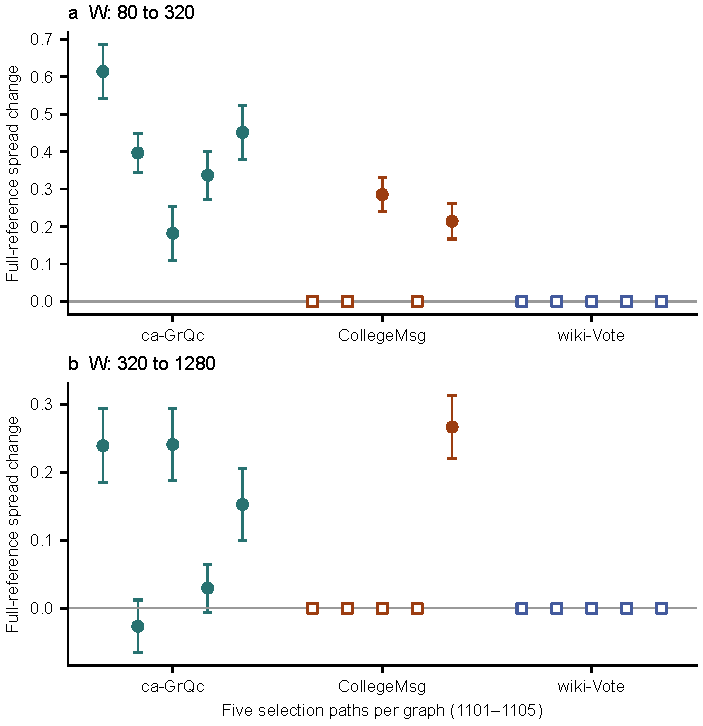
\includegraphics[width=\linewidth]{Fig2.pdf}
\caption{Reference-set changes and independent spread changes. Filled circles denote changed final sets; hollow squares denote unchanged sets. Paths 1101--1105 run from left to right within each graph. Bars are unadjusted 95\% conditional Monte Carlo intervals from 10,000 paired worlds. Panel-specific vertical scales reveal small changes; the intervals condition on selected sets and do not describe variation across networks.}\label{fig:transitions}
\end{figure}

\subsection{Quality determines the value of computational savings}
Degree-4k reduces measured selection time by 98.40--99.67\% at $W=1280$ while reproducing all full-reference trajectories (Table~\ref{tab:cost}). Including setup, both world families and independent evaluation gives estimated savings of \CollegeDegreeSaving{}--\WikiDegreeSaving{}\%. The difference between these ranges shows why the timing scope matters.
\begin{table}[htbp]
\caption{Degree-4k cost at $W=1280$, averaged over five paths. Full and degree columns give measured selection time. Verification savings include separately measured setup plus world preparation, selection and evaluation; they are assembled estimates.}\label{tab:cost}
\begin{tabular}{lrrrr}
\toprule
Graph & Full (s) & Degree (s) & Saving (\%) & Verify saving (\%) \\
\midrule
ca-GrQc & 23.53 & 0.109 & 99.54 & 92.77 \\
CollegeMsg & 5.89 & 0.094 & 98.40 & 86.59 \\
wiki-Vote & 158.94 & 0.520 & 99.67 & 96.26 \\
\bottomrule
\end{tabular}
\end{table}


Descriptive loss thresholds further separate speed from utility preservation. At $W=1280$, degree-4k meets the zero point-estimate loss threshold on every path. Default PageRank-4k meets 10\% on ca-GrQc and CollegeMsg, but fails 20\% on every wiki-Vote path. None of the random-pool path means meets 20\%. Online Resource 1 reports all six frozen thresholds (0, 1, 2.5, 5, 10 and 20\%) and their cost estimates; these are descriptive criteria rather than application-validated tolerances.

The fixed-edge control retains the main PageRank loss pattern at $W=320$, with mean differences of $-0.16240$, $-0.93417$ and $-40.57597$ nodes on ca-GrQc, CollegeMsg and wiki-Vote. Degree-4k reproduces 1/3, 3/3 and 3/3 corresponding trajectories. Thus coupling changes some reference-agreement outcomes even when the prominent utility losses persist. Complete control paths and repeated timings are supplied in Online Resource 1.
\FloatBarrier

\section{Discussion}
The results show why reference budget and numerical ranking precision should be controlled separately. Increasing the selection budget changes the sampled greedy computation; tightening ranking tolerance can change which vertices enter that computation. On ca-GrQc, a two-candidate exchange removes the default quality reversal while leaving budget-dependent seed changes. On the directed graphs, tighter ranking preserves the losses. Evaluating only one resolution would merge these different explanations.

Three reporting choices follow. First, report the candidate fraction and actual ranking tolerance alongside the reference budget. Second, distinguish ordered agreement, final-set agreement and independently evaluated utility, including both conditional uncertainty and path variation. Third, state which stages a cost comparison includes. Together these quantities show whether a restriction preserves a reference computation, retains its spread, or merely reduces search time.

The evidence covers three selected external networks under $k=5$, $p=.01$, $h=3$ and selection budgets up to 1280. The five paths are computational replicates; the graphs do not form a probability sample of social systems. Observed messages, coauthorships and votes provide topology, not calibrated causal diffusion. Other seed budgets, propagation laws, edge probabilities and orientations may change the results. Reference agreement does not establish expected-optimality or convergence, and the paired numerical control remains post-hoc. Finally, cost savings are relative to exhaustive selection in this implementation; assembled verification costs exclude cold-start overhead. These boundaries define where further validation is needed.

\section{Conclusion}
Candidate-restriction quality depends on both the finite greedy reference and the precision of the truncated ranking. Our paired evaluation identifies a solver-sensitive budget reversal, tests its external scope, and separates seed-set changes from utility and cost. Degree-based pools reproduce all highest-budget external references at substantially lower selection cost, while PageRank's precision and topology sensitivity qualify its earlier small-graph agreement. Reporting these quantities together makes quality--cost conclusions interpretable and reproducible.

\paragraph{Supplementary information.} Online Resource 1 contains the complete result matrix, coverage and direction diagnostics, precision and transition tables, loss--cost curves, coupling controls and reproducibility details.
\section*{Statements and Declarations}
\paragraph{Funding.} This work was supported by a provincial undergraduate innovation and entrepreneurship training project.
\paragraph{Competing interests.} The authors declare that they have no competing interests.
\paragraph{Author contributions.} Jiayue Sun: conceptualization, methodology, software, validation, formal analysis, investigation, data curation, visualization, and writing---original draft. Binbin Yong: supervision, methodology, project administration, and writing---review and editing. Junjie An: software, data curation, and writing---review and editing. Tianyu Bo: validation, visualization, and writing---review and editing. Shuai Li: formal analysis, validation, and writing---review and editing. All authors read and approved the final manuscript and agreed to its submission to \textit{Computing}.
\paragraph{Data availability.} The third-party datasets are available from the cited providers under their access terms and are not redistributed. Source records, expected SHA-256 hashes and preprocessing instructions accompany the submission.
\paragraph{Code availability.} Frozen source snapshots, configurations, validators, analysis scripts, condition-level outputs and figure-source tables are supplied with the submission for editorial and peer-review access.
\begin{thebibliography}{99}
\bibitem{ref1} Kempe D, Kleinberg J, Tardos É (2003) Maximizing the spread of influence through a social network. In: ACM SIGKDD, pp 137--146. \url{https://doi.org/10.1145/956750.956769}

\bibitem{ref2} Tang Y, Shi Y, Xiao X (2015) Influence maximization in near-linear time: a martingale approach. In: ACM SIGMOD, pp 1539--1554. \url{https://doi.org/10.1145/2723372.2723734}

\bibitem{ref8} Cheng S, Shen H, Huang J, Zhang G, Cheng X (2013) StaticGreedy: solving the scalability-accuracy dilemma in influence maximization. In: CIKM, pp 509--518. \url{https://doi.org/10.1145/2505515.2505541}

\bibitem{ref9} Li Y, Fan J, Wang Y, Tan K-L (2018) Influence maximization on social graphs: a survey. IEEE Transactions on Knowledge and Data Engineering 30:1852--1872. \url{https://doi.org/10.1109/TKDE.2018.2807843}

\bibitem{ref16} Arora A, Galhotra S, Ranu S (2017) Debunking the myths of influence maximization: an in-depth benchmarking study. In: SIGMOD, pp 651--666. \url{https://doi.org/10.1145/3035918.3035924}

\bibitem{ref7} Leskovec J, Krause A, Guestrin C, Faloutsos C, VanBriesen J, Glance N (2007) Cost-effective outbreak detection in networks. In: KDD, pp 420--429. \url{https://doi.org/10.1145/1281192.1281239}

\bibitem{ref12} Rui X, Yang X, Fan J, Wang Z (2020) A neighbour scale fixed approach for influence maximization in social networks. Computing 102:427--449. \url{https://doi.org/10.1007/s00607-019-00778-5}

\bibitem{ref13} Fan C, Wang Z, Zhang J, Zhao J, Rui X (2024) Influence maximization in social networks based on discrete harris hawks optimization algorithm. Computing 106:327--351. \url{https://doi.org/10.1007/s00607-023-01207-4}

\bibitem{ref19} Ko J, Kim S, Lee K, et al. (2025) Inductive influence estimation and maximization over unseen social networks under two diffusion models. Data Mining and Knowledge Discovery 39:55. \url{https://doi.org/10.1007/s10618-025-01137-z}

\bibitem{ref11} Yanchenko E, Murata T, Holme P (2024) Influence maximization on temporal networks: a review. Applied Network Science 9:16. \url{https://doi.org/10.1007/s41109-024-00625-3}

\bibitem{ref15} Aral S, Dhillon PS (2018) Social influence maximization under empirical influence models. Nature Human Behaviour 2:375--382. \url{https://doi.org/10.1038/s41562-018-0346-z}

\bibitem{networkxpr} NetworkX developers (2025) PageRank, NetworkX 3.5 documentation. \url{https://networkx.org/documentation/networkx-3.5/reference/algorithms/generated/networkx.algorithms.link_analysis.pagerank_alg.pagerank.html}. Accessed 15 October 2026

\bibitem{snap} Leskovec J, Krevl A (2014) SNAP datasets: Stanford large network dataset collection. \url{https://snap.stanford.edu/data}. Accessed 15 October 2026

\bibitem{college} Panzarasa P, Opsahl T, Carley KM (2009) Patterns and dynamics of users' behavior and interaction: Network analysis of an online community. Journal of the American Society for Information Science and Technology 60:911--932. \url{https://doi.org/10.1002/asi.21015}

\bibitem{grqc} Leskovec J, Kleinberg J, Faloutsos C (2007) Graph evolution: densification and shrinking diameters. ACM Transactions on Knowledge Discovery from Data 1(1):2. \url{https://doi.org/10.1145/1217299.1217301}

\bibitem{signed} Leskovec J, Huttenlocher D, Kleinberg J (2010) Signed networks in social media. In: CHI, pp 1361--1370. \url{https://doi.org/10.1145/1753326.1753532}

\bibitem{links} Leskovec J, Huttenlocher D, Kleinberg J (2010) Predicting positive and negative links in online social networks. In: WWW, pp 641--650. \url{https://doi.org/10.1145/1772690.1772756}

\bibitem{ref3} Génois M, Vestergaard CL, Fournet J, Panisson A, Bonmarin I, Barrat A (2015) Data on face-to-face contacts in an office building suggest a low-cost vaccination strategy based on community linkers. Network Science 3:326--347. \url{https://doi.org/10.1017/nws.2015.10}

\bibitem{ref4} Génois M, Barrat A (2018) Can co-location be used as a proxy for face-to-face contacts? EPJ Data Science 7:11. \url{https://doi.org/10.1140/epjds/s13688-018-0140-1}

\bibitem{ref5} Cattuto C, Van den Broeck W, Barrat A, Colizza V, Pinton J-F, Vespignani A (2010) Dynamics of person-to-person interactions from distributed RFID sensor networks. PLoS ONE 5:e11596. \url{https://doi.org/10.1371/journal.pone.0011596}

\bibitem{ref6} Kiti MC, Tizzoni M, Kinyanjui TM, et al. (2016) Quantifying social contacts in a household setting of rural Kenya using wearable proximity sensors. EPJ Data Science 5:21. \url{https://doi.org/10.1140/epjds/s13688-016-0084-2}

\bibitem{ref17} Barabasi A-L, Albert R (1999) Emergence of scaling in random networks. Science 286:509--512. \url{https://doi.org/10.1126/science.286.5439.509}

\bibitem{ref18} Holland PW, Laskey KB, Leinhardt S (1983) Stochastic blockmodels: first steps. Social Networks 5:109--137. \url{https://doi.org/10.1016/0378-8733(83)90021-7}
\end{thebibliography}

\end{document}
